%!TeX program = lualatex
\documentclass[10pt, aspectratio=169, t]{beamer}
% ---------------------------------------------------------------------
% 1. PACKAGES
% ---------------------------------------------------------------------

\usepackage{physics}
%% siunitx loads after physics and therefore leaves \qty alone: here \qty is
%% the physics one (auto-sized fences).  Quantities go through \SI{<num>}{<unit>}
%% -- \qty{540}{\second} silently becomes (540)(\second) and errors on \second.
\usepackage{siunitx}
\usepackage{fontspec}
\usepackage{unicode-math}
\usepackage{tikz}
\usepackage{pgfplots}
\usepackage{tcolorbox}
\usepackage{booktabs}
\usepackage{animate} % Essential for scientific animations
\usepackage{multimedia}
\usepackage{graphicx}
\usepackage{hyperref}
\usepackage{subcaption}
\usepackage{listings}
\usepackage{microtype}
\usepackage{xspace}     % needed by the \eg / \ie macros in macros.tex
\usepackage{amsmath}
\usepackage{amsfonts}
\usepackage{amssymb}
\usepackage{mathtools} % \overbracket and friends (needed by the \btdot/\btring macros)
\usepackage{accents}   % \accentset (needed by the \tdot/\tring macros)
\usepackage[bbgreekl]{mathbbol}
\usepackage{eqnlines}

\pgfplotsset{compat=1.18}
\tcbuselibrary{skins, breakable}

\definecolor{PaperBg}{HTML}{F9F9F9} 
\definecolor{SumiInk}{HTML}{181616} 
\definecolor{DragonRed}{HTML}{C34043}   
\definecolor{DragonGold}{HTML}{C0A36E}  % Secondary (Highlights)
\definecolor{DragonTeal}{HTML}{6A9589}  % Tertiary (Code/Figures)
\definecolor{DragonGray}{HTML}{727169}  % Metadata/Comments
\definecolor{DragonIndigo}{HTML}{7E78A0} % New: For Math/Theorems
\definecolor{DragonRed}{HTML}{C34043}    % Existing: For Frame Headings

% ---------------------------------------------------------------------
% 3. TYPOGRAPHY
% ---------------------------------------------------------------------
\setmainfont{Fira Sans}
\setsansfont{Fira Sans}
\setmathfont{Garamond-Math} 
\setmathfont{STIX Two Math}[range={bb,bbit}, Scale=MatchUppercase] % Fix for \mathbb
\setmonofont{JetBrains Mono}[Scale=0.85, Color=SumiInk]

% ---------------------------------------------------------------------
% 4. MINIMALIST THEME SETUP
% ---------------------------------------------------------------------
\setbeamercolor{background canvas}{bg=PaperBg}
\setbeamercolor{normal text}{fg=SumiInk}
\setbeamercolor{frametitle}{fg=DragonRed}
\setbeamercolor{structure}{fg=DragonRed}

\setbeamertemplate{navigation symbols}{}

% Elegant Frametitle (Text only, no bar)
\setbeamertemplate{frametitle}{
    \vspace*{0.6cm}
    \bfseries\Large\insertframetitle
    \par
    % Optional: Subtle underline
    % \vspace*{0.1cm}\hrule\color{DragonGray!20}
}

% Minimal Footer (Just page number, bottom right)
\setbeamertemplate{footline}{
    \hfill \color{DragonGray}\scriptsize\insertframenumber \hspace{0.5cm} \vspace{0.3cm}
}

% ---------------------------------------------------------------------
% 5. SLEEK BLOCKS (The "Left-Line" Style)
% ---------------------------------------------------------------------

\newtcolorbox{math-block}[1]{
    enhanced,
    frame hidden,           % No box border
    colback=PaperBg,        % Blends with background
    borderline west={2pt}{0pt}{DragonIndigo}, % The "Dragon" touch
    title={\bfseries\color{DragonIndigo}#1}, % Colored Title
    detach title,
    before upper={\tcbtitle\par\vspace{0.2em}},
    coltext=SumiInk,
    left=10pt,
    sharp corners
}

\newtcolorbox{code-block}[1]{
    enhanced,
    frame hidden,
    colback=PaperBg, % Keep it clean, or use {DragonGray!5} for slight shading
    borderline west={2pt}{0pt}{DragonTeal},
    title={\small\ttfamily\color{DragonTeal}#1},
    detach title,
    before upper={\tcbtitle\par\vspace{0.1em}},
    left=10pt,
    sharp corners
}

% ---------------------------------------------------------------------
% 6. CODE STYLING
% ---------------------------------------------------------------------
\lstset{
    basicstyle=\ttfamily\footnotesize\color{SumiInk},
    keywordstyle=\bfseries\color{DragonRed},
    commentstyle=\itshape\color{DragonGray},
    stringstyle=\color{DragonTeal},
    numbers=none,
    frame=none,
    backgroundcolor=\color{PaperBg}
}

% Add this to preamble.tex
\AtBeginSection[]{
  \begin{frame}[plain]
    \centering
    \vspace*{\fill}
    \usebeamerfont{title}
    \color{DragonTeal}\Huge \insertsectionhead\par
    \vspace*{\fill}
  \end{frame}
}

% ---------------------------------------------------------------------
% 8. USER MACROS
% ---------------------------------------------------------------------
% Must come last: the macros use the colors and packages defined above.
%% User macros
\DeclareMathOperator{\sym}{sym}
\DeclareMathOperator{\asym}{asym}
\DeclareMathOperator{\cof}{cof}
\DeclareMathOperator{\laplace}{\bigtriangleup}
\newcommand{\tensorq}[1]{\symbb{#1}}      % tensorial quantity
\newcommand{\identityM}{\ensuremath{\tensorq{I}}}
\newcommand{\fgrad}{\tensorq{F}}
\newcommand{\detf}{\det\, \fgrad}
\newcommand{\vgrad}{\tensorq{L}}
\newcommand{\symvgrad}{\tensorq{D}}
\newcommand{\asymvgrad}{\mathbb{\omega}}
\newcommand{\cstress}{\tensorq{T}}
\newcommand{\pkstress}{\tensorq{T}_{\mathrm{R}}}
\newcommand{\spkstress}{\tensorq{S}_{\mathrm{R}}}
\newcommand{\rcg}{\tensorq{C}}
\newcommand{\lcg}{\tensorq{B}}
% \mdv[<species>]{<quantity>}:
% - \mdv                -> \dfrac{\mathrm{D}}{\mathrm{D}t}
% - \mdv{v}             -> \dfrac{\mathrm{D} v}{\mathrm{D}t}
% - \mdv[a]{v}          -> \dfrac{\mathrm{D}_{a} v}{\mathrm{D}t}
% - \mdv[a]             -> \dfrac{\mathrm{D}_{a}}{\mathrm{D}t}
\NewDocumentCommand{\mdv}{o g}{%
  \IfNoValueTF{#2}{% no braced arg -> operator form
    \IfValueTF{#1}
      {\dfrac{\mathrm{D}_{#1}}{\mathrm{D}t}}% species subscript on operator
      {\dfrac{\mathrm{D}}{\mathrm{D}t}}% plain operator
  }{% braced arg present -> numerator form
    \IfValueTF{#1}
      {\dfrac{\mathrm{D}_{#1} #2}{\mathrm{D}t}}% \mdv[a]{v}
      {\dfrac{\mathrm{D} #2}{\mathrm{D}t}}% \mdv{v}
  }%
}

%% ---------------------------------------------------------------------
%% Math-mode scaling/raising helpers
%% ---------------------------------------------------------------------
%% Ported from the thesis (`preamble/math/macros.tex`). Both pick the right size
%% for the current math style via \mathpalette, so accents built on top of them
%% shrink correctly in scripts and subscripts.
\NewDocumentCommand{\raisemath}{m}{\mathpalette{\raisemathAux{#1}}}        % \raisemath{<len>}{...}
\NewDocumentCommand{\raisemathAux}{mmm}{\raisebox{#1}{\(#2#3\)}}
\NewDocumentCommand{\scalemath}{m O{}}{\mathpalette{\scalemathAux{#1}[#2]}} % \scalemath{<x>}[<y>]{...}
\NewDocumentCommand{\scalemathAux}{m O{} mm}{%
    \IfBlankTF{#2}{\scalebox{#1}{\(#3#4\)}}{\scalebox{#1}[#2]{\(#3#4\)}}%
}

%% ---------------------------------------------------------------------
%% Time derivatives and objective rates
%% ---------------------------------------------------------------------
%% Ported from ~/Templates/homework/preamble/math/macros.tex, adapted for
%% unicode-math:
%%   - \bm{\cdot} -> \symbf{\cdot}  (bm must not be used together with unicode-math)
%%   - \overbracket takes NO optional arguments here: unicode-math overrides the
%%     mathtools version with a stretchy Unicode accent.
%%
%%   \tdot{\vb{v}}       -> single overdot        (material/time derivative)
%%   \tddot{\vb{x}}      -> double overdot        (second time derivative)
%%   \btdot{\rho\theta}  -> overbracket + overdot (derivative of a whole group)
%%   \tring{\tensorq{A}} -> objective rate ring
%%   \btring{...}        -> overbracket + ring
%%   \wring{...}         -> overline + ring
\NewDocumentCommand{\tdotsymbol}{}{\scalemath{1.5}{\symbf{\cdot}}}
\NewDocumentCommand{\tringsymbol}{}{\scalemath{0.9}{\circ}}

%% Gap between the two dots of \tddot. Garamond-Math has a narrow \cdot, so the
%% thesis value (-3mu, tuned for Latin Modern) merges them into a single blob.
\NewDocumentCommand{\tddotsep}{}{-1mu}

\NewDocumentCommand{\tdot}{m}{%
    \accentset{\raisemath{-0.15ex}{\tdotsymbol}}{#1}%
}
\NewDocumentCommand{\tddot}{O{\tddotsep} m}{%
    \accentset{\raisemath{-0.15ex}{\scalemath{1.5}{\symbf{\cdot}\mspace{#1}\symbf{\cdot}}}}{#2}%
}
\NewDocumentCommand{\btdot}{m}{%
    \accentset{\raisemath{-0.15ex}{\tdotsymbol}}{\overbracket{#1}}%
}
\NewDocumentCommand{\tring}{m}{%
    \accentset{\raisemath{-0.15ex}{\tringsymbol}}{#1}%
}
\NewDocumentCommand{\btring}{m}{%
    \accentset{\raisemath{-0.15ex}{\tringsymbol}}{\overbracket{#1}}%
}
\NewDocumentCommand{\wring}{m}{%
    \accentset{\raisemath{-0.15ex}{\tringsymbol}}{\overline{#1}}%
}

%% ---------------------------------------------------------------------
%% Equation annotations
%% ---------------------------------------------------------------------
%% A short description hung to the right of one line of a `columns` equations
%% block. Open the annotation column with an extra `&`, exactly like alignat:
%%
%%   \begin{math-block}{System of equations}
%%       \begin{equations}[columns,*]
%%           \rho \dv{\vb{v}}{t} &= -\grad p + \rho \vb{g}, && \eqnote{momentum balance} \\
%%           \dv{\theta}{t}      &= 0,                      && \eqnote{isentropic evolution}
%%       \end{equations}
%%   \end{math-block}
%%
%% All annotations in one block line up automatically -- eqnlines treats the
%% extra column like any other alignment column.
%%
%%   \eqnote{text}       normal: a \quad of air, then small gray text
%%   \eqnote*{text}      no leading \quad (when the column is already far enough right)
%%   \eqnote[7em]{text}  wrap the text in a top-aligned parbox of the given width
\NewDocumentCommand{\eqnote}{s o m}{%
    \text{%
        \IfBooleanF{#1}{\quad}%
        \normalfont\footnotesize\color{DragonGray}%
        \IfValueTF{#2}
            {\parbox[t]{#2}{\raggedright #3}}
            {#3}%
    }%
}

%% ---------------------------------------------------------------------
%% Latin abbreviations
%% ---------------------------------------------------------------------
%% Same definitions as the thesis (`preamble/user/macros.tex`): American
%% academic style, i.e. always a trailing comma, and \xspace so a following
%% space is kept without needing `\eg\ ` or `\eg{}`.
%%   \eg some example   ->  "e.g., some example"
%%   \ie a restatement  ->  "i.e., a restatement"
\newcommand{\eg}{e.g.,\xspace}   % exempli gratia -- non-exhaustive example
\newcommand{\ie}{i.e.,\xspace}   % id est         -- clarification/restatement

%% Cancel macro
\definecolor{cancelgray}{gray}{0.85}
\tikzset{
    main node/.style={inner sep=0,outer sep=0},
    label node/.style={inner sep=0.3em,font=\tiny,overlay},
    strike out/.style={shorten <=-.2em,shorten >=-.2em,overlay,thick,double distance = 0em,line cap=round},
}
\NewDocumentCommand{\cancel}{O{cancelgray}mo}{%
    \tikz[baseline=(N.base)]{
        \node[main node](N){\(#2\)};
        \IfValueT{#3}{\node[label node, gray, anchor=south] at (N.north){#3};}
        \draw[strike out, #1]  (N.south west) -- (N.north east);
    }
}

%% ---------------------------------------------------------------------
%% Linking related items on a slide
%% ---------------------------------------------------------------------
%% \link[<keys>]{<stuff>} paints a phrase and the symbol it refers to in the
%% same colour, so the eye ties the two together without an arrow or an extra
%% sentence.  Everything sharing a <thread> name shares a colour; each new
%% thread takes the next colour off \g_belan_link_palette_seq, in order of first
%% use, so several independent threads can live on one frame:
%%
%%   \item poor conservation with \link[h]{adaptive $h$},
%%   ...  w_{ab}\left(\link[h]{h_a}\right)  ...          % same gold
%%   \item conservation via the $\link[f]{\grad h}$ terms $\link[f]{f_a}$,
%%   ...  \frac{\link[f]{f_a} P_a}{P_a^{2/\gamma}}  ...  % teal, second thread
%%
%% The optional argument is a key=value list, but a bare word that is not one of
%% the keys below is still read as the thread name, so the short form keeps
%% working: \link{x} uses the thread `main', \link[h]{x} the thread `h', and a
%% name that *is* a defined colour is taken literally, so \link[DragonRed]{x}
%% remains a one-off override.
%%
%% Keys:
%%   thread=<name>   thread whose colour to use (default `main'); same as the
%%                   bare form, but needed when the name clashes with a key
%%   color=<colour>  paint with this colour and skip the thread bookkeeping;
%%                   any xcolor expression works (color=DragonRed!60!SumiInk)
%%   mix=<0-100>     strength of the *text* colour, blended towards `bg':
%%                   mix=45 fades a thread that should stay legible but quiet
%%                   (default 100 = the thread colour as is)
%%   bg=<colour>     what mix and tint blend into (default PaperBg, i.e. the
%%                   slide background -- set it on a coloured block)
%%   bold            embolden the argument as well (\textbf / \symbf)
%%   box             tinted rounded background behind the argument
%%   frame           thin outline in the thread colour
%%   under           coloured rule just under the baseline
%%   tint=<0-100>    strength of the `box' fill (default 15)
%%   plain           leave the text in the running colour and only decorate;
%%                   pairs with box/under when full colouring is too loud
%%   on=<overlay>    beamer overlay spec: the colour and the decorations appear
%%                   only on those slides, the text is untouched elsewhere
%%                   (\link[h,on=2-]{h_a}).  The quiet slides still reserve the
%%                   padding of box/frame, so the line does not reflow when the
%%                   highlight arrives -- a gated `bold' does move things, though
%%   name=<node>     also drop a remembered tikz node of that name around the
%%                   argument, so a later \tikz[remember picture,overlay] can
%%                   draw an arrow to it (costs the usual two extra runs)
%%
%% Thread bookkeeping and document-wide defaults:
%%   \setlinkcolor{<thread>}{<colour>}   pin a thread instead of letting the
%%                                       palette assign it (before first use)
%%   \setlinkpalette{<c1,c2,...>}        replace the auto-assignment cycle
%%   \setlinkstyle{<keys>}               keys applied to every later \link,
%%                                       overridden per call (\setlinkstyle{under}
%%                                       makes the whole talk underline instead
%%                                       of recolour)
%%
%% Works in both modes: in math the argument stays math, so \link[h]{h_a} still
%% typesets as h_a.  The colour is applied inside a group, which makes the
%% argument a single Ord atom -- wrap symbols and subformulae with it, not
%% relations or operators, or the surrounding math spacing shifts.  The
%% decorating keys (box/frame/under/name) put the argument in a tikz node, which
%% is an Ord atom too, but it does freeze the size: a \link[box]{...} inside
%% \left(...\right) will not grow with the fence.
%%
%% The palette colours are darkened towards SumiInk: the raw Dragon hues are
%% pale on PaperBg and wash out on a projector.
\colorlet{LinkGold}{DragonGold!75!SumiInk}
\colorlet{LinkTeal}{DragonTeal!85!SumiInk}
\colorlet{LinkIndigo}{DragonIndigo!90!SumiInk}
\colorlet{LinkRed}{DragonRed}

%% Overlay gate, kept out of \ExplSyntaxOn so beamer sees a literal `<' spec.
\newcommand{\belanLinkAlt}[3]{\alt<#1>{#2}{#3}}

%% Node wrapper, likewise kept out of \ExplSyntaxOn: tikz parses its own
%% arguments and is happier with catcodes it recognises.
%%   #1 picture options   #2 node options   #3 underline colour (empty: none)
%%   #4 content, already coloured and back in the right mode
\newcommand{\belanLinkNode}[4]{%
    \tikz[baseline=(belanlink.base)#1]{%
        \node[#2](belanlink){#4};%
        \if\relax\detokenize{#3}\relax\else
            \draw[#3,line width=0.6pt]
                ([yshift=-0.22em]belanlink.base-|belanlink.west) --
                ([yshift=-0.22em]belanlink.base-|belanlink.east);%
        \fi
    }%
}

\ExplSyntaxOn
\prop_new:N \g_belan_link_prop          % thread name -> colour
\seq_new:N  \g_belan_link_palette_seq   % colours handed out, in order
\int_new:N  \g_belan_link_int           % how many threads are already assigned
\tl_new:N   \g_belan_link_style_tl      % keys prepended to every call

\tl_new:N   \l_belan_link_thread_tl
\tl_new:N   \l_belan_link_given_tl      % colour= , empty when unused
\tl_new:N   \l_belan_link_color_tl      % resolved thread colour
\tl_new:N   \l_belan_link_text_tl       % ... after the mix= blend
\tl_new:N   \l_belan_link_bg_tl
\tl_new:N   \l_belan_link_on_tl
\tl_new:N   \l_belan_link_name_tl
\tl_new:N   \l_belan_link_opts_tl
\tl_new:N   \l_belan_link_pic_tl
\int_new:N  \l_belan_link_tint_int
\int_new:N  \l_belan_link_mix_int
\bool_new:N \l_belan_link_bold_bool
\bool_new:N \l_belan_link_box_bool
\bool_new:N \l_belan_link_frame_bool
\bool_new:N \l_belan_link_under_bool
\bool_new:N \l_belan_link_plain_bool
\bool_new:N \l_belan_link_math_bool   % mode at the call site, sampled once
\bool_new:N \l_belan_link_off_bool    % an on=<spec> link, on a slide it is off

\seq_gset_from_clist:Nn \g_belan_link_palette_seq
    { LinkGold , LinkTeal , LinkIndigo , LinkRed }

\keys_define:nn { belan / link }
  {
    thread    .tl_set:N    = \l_belan_link_thread_tl ,
    color     .tl_set:N    = \l_belan_link_given_tl ,
    colour    .tl_set:N    = \l_belan_link_given_tl ,
    bg        .tl_set:N    = \l_belan_link_bg_tl ,
    on        .tl_set:N    = \l_belan_link_on_tl ,
    name      .tl_set:N    = \l_belan_link_name_tl ,
    tint      .int_set:N   = \l_belan_link_tint_int ,
    mix       .int_set:N   = \l_belan_link_mix_int ,
    bold      .bool_set:N  = \l_belan_link_bold_bool ,
    bold      .default:n   = true ,
    box       .bool_set:N  = \l_belan_link_box_bool ,
    box       .default:n   = true ,
    frame     .bool_set:N  = \l_belan_link_frame_bool ,
    frame     .default:n   = true ,
    under     .bool_set:N  = \l_belan_link_under_bool ,
    under     .default:n   = true ,
    underline .bool_set:N  = \l_belan_link_under_bool ,
    underline .default:n   = true ,
    plain     .bool_set:N  = \l_belan_link_plain_bool ,
    plain     .default:n   = true ,
    %% anything else is the thread name -- this is what keeps \link[h]{...}
    %% and \link[DragonRed]{...} working after the switch to key=value.
    unknown   .code:n      = { \tl_set:Nx \l_belan_link_thread_tl { \l_keys_key_str } } ,
  }

%% Per-call state: the keys are set inside a group, but the defaults have to be
%% re-established explicitly because \setlinkstyle may have moved them.
\cs_new_protected:Npn \belan_link_reset:
  {
    \tl_set:Nn \l_belan_link_thread_tl { main }
    \tl_clear:N \l_belan_link_given_tl
    \tl_set:Nn \l_belan_link_bg_tl { PaperBg }
    \tl_clear:N \l_belan_link_on_tl
    \tl_clear:N \l_belan_link_name_tl
    \int_set:Nn \l_belan_link_tint_int { 15 }
    \int_set:Nn \l_belan_link_mix_int  { 100 }
    \bool_set_false:N \l_belan_link_bold_bool
    \bool_set_false:N \l_belan_link_box_bool
    \bool_set_false:N \l_belan_link_frame_bool
    \bool_set_false:N \l_belan_link_under_bool
    \bool_set_false:N \l_belan_link_plain_bool
    \bool_set_false:N \l_belan_link_off_bool
  }

%% True when the name is *not* a defined colour, i.e. when it names a thread.
%% \@ifundefinedcolor{<name>}{<undefined>}{<defined>}; \ExplSyntaxOn gives @
%% catcode 12, hence \use:c.
\cs_new_protected:Npn \belan_link_if_thread:nTF #1#2#3
  { \use:c { @ifundefinedcolor } {#1} {#2} {#3} }

%% Hand the next palette colour to a thread never seen before; wrap around when
%% the palette runs out rather than erroring.
\cs_new_protected:Npn \belan_link_assign:n #1
  {
    \int_gincr:N \g_belan_link_int
    \prop_gput:Nnx \g_belan_link_prop {#1}
      {
        \seq_item:Nn \g_belan_link_palette_seq
          {
            \int_mod:nn { \g_belan_link_int - 1 }
                        { \seq_count:N \g_belan_link_palette_seq } + 1
          }
      }
  }

\cs_new_protected:Npn \belan_link_resolve:
  {
    \tl_if_empty:NTF \l_belan_link_given_tl
      {
        \exp_args:NV \belan_link_if_thread:nTF \l_belan_link_thread_tl
          {   % not a colour name -> a thread
            \prop_if_in:NVF \g_belan_link_prop \l_belan_link_thread_tl
              { \exp_args:NV \belan_link_assign:n \l_belan_link_thread_tl }
            \prop_get:NVN \g_belan_link_prop \l_belan_link_thread_tl
              \l_belan_link_color_tl
          }
          { \tl_set_eq:NN \l_belan_link_color_tl \l_belan_link_thread_tl }
      }
      { \tl_set_eq:NN \l_belan_link_color_tl \l_belan_link_given_tl }
    %% mix=100 is left alone: `<expr>!100!<bg>' is not a legal xcolor
    %% expression when <expr> already carries a `!'.
    \int_compare:nNnTF \l_belan_link_mix_int = { 100 }
      { \tl_set_eq:NN \l_belan_link_text_tl \l_belan_link_color_tl }
      {
        \tl_set:Nx \l_belan_link_text_tl
          {
            \l_belan_link_color_tl ! \int_use:N \l_belan_link_mix_int
            ! \l_belan_link_bg_tl
          }
      }
  }

%% The content, bolded and coloured.  The mode is read from
%% \l_belan_link_math_bool, sampled before anything is opened: inside a tikz
%% node TeX is in text mode again, so \mode_if_math: would answer for the node,
%% not for the call site.
\cs_new_protected:Npn \belan_link_body:n #1
  {
    \bool_if:NTF \l_belan_link_plain_bool
      { \belan_link_bold:n {#1} }
      {
        \bool_if:NTF \l_belan_link_math_bool
          { { \exp_args:NV \color \l_belan_link_text_tl \belan_link_bold:n {#1} } }
          { \exp_args:NV \textcolor \l_belan_link_text_tl { \belan_link_bold:n {#1} } }
      }
  }

\cs_new_protected:Npn \belan_link_bold:n #1
  {
    \bool_if:NTF \l_belan_link_bold_bool
      { \bool_if:NTF \l_belan_link_math_bool { \symbf {#1} } { \textbf {#1} } }
      {#1}
  }

%% box / frame / under / name all need a node; everything is hung on the one
%% node `belanlink' so the underline can be measured from its baseline.  A math
%% argument goes back into math with \ensuremath, since the node body is text.
\cs_new_protected:Npn \belan_link_node:n #1
  {
    \tl_set:Nn \l_belan_link_opts_tl { outer~sep=0pt }
    \bool_lazy_or:nnTF { \l_belan_link_box_bool } { \l_belan_link_frame_bool }
      {
        \tl_put_right:Nn \l_belan_link_opts_tl
          { ,inner~xsep=0.22em,inner~ysep=0.12em,rounded~corners=1.5pt }
      }
      { \tl_put_right:Nn \l_belan_link_opts_tl { ,inner~sep=0pt } }
    \bool_lazy_and:nnT { \l_belan_link_box_bool } { ! \l_belan_link_off_bool }
      {
        \tl_put_right:Nx \l_belan_link_opts_tl
          {
            ,fill= \l_belan_link_color_tl ! \int_use:N \l_belan_link_tint_int
                   ! \l_belan_link_bg_tl
          }
      }
    \bool_lazy_and:nnT { \l_belan_link_frame_bool } { ! \l_belan_link_off_bool }
      {
        \tl_put_right:Nx \l_belan_link_opts_tl
          { ,draw= \l_belan_link_color_tl ,line~width=0.4pt }
      }
    \tl_clear:N \l_belan_link_pic_tl
    \tl_if_empty:NF \l_belan_link_name_tl
      {
        \tl_put_right:Nx \l_belan_link_opts_tl { ,alias= \l_belan_link_name_tl }
        \tl_set:Nn \l_belan_link_pic_tl { ,remember~picture }
      }
    \use:x
      {
        \exp_not:N \belanLinkNode
          { \l_belan_link_pic_tl }
          { \l_belan_link_opts_tl }
          {
            \bool_lazy_and:nnT { \l_belan_link_under_bool } { ! \l_belan_link_off_bool }
              { \l_belan_link_color_tl }
          }
      }
      {
        \bool_if:NTF \l_belan_link_math_bool
          { \ensuremath { \belan_link_body:n {#1} } }
          { \belan_link_body:n {#1} }
      }
  }

\cs_new_protected:Npn \belan_link_render:n #1
  {
    \bool_lazy_any:nTF
      {
        { \l_belan_link_box_bool }
        { \l_belan_link_frame_bool }
        { \l_belan_link_under_bool }
        { ! \tl_if_empty_p:N \l_belan_link_name_tl }
      }
      { \belan_link_node:n {#1} }
      { \belan_link_body:n {#1} }
  }

%% on=<spec>: styled on those overlays, quiet everywhere else.  The quiet branch
%% still builds the node, so the padding of box/frame is reserved on every slide
%% and the line does not reflow when the highlight switches on; only `bold' can
%% still move things, since bolding is a change of width.
\cs_new_protected:Npn \belan_link_gate:n #1
  {
    \tl_if_empty:NTF \l_belan_link_on_tl
      { \belan_link_render:n {#1} }
      {
        \use:x { \exp_not:N \belanLinkAlt { \l_belan_link_on_tl } }
          { \belan_link_render:n {#1} }
          { \belan_link_render_off:n {#1} }
      }
  }

%% The `off' slides of an on=<spec> link: geometry kept, every colour dropped.
\cs_new_protected:Npn \belan_link_render_off:n #1
  {
    \bool_set_true:N  \l_belan_link_off_bool
    \bool_set_true:N  \l_belan_link_plain_bool
    \bool_set_false:N \l_belan_link_bold_bool
    \belan_link_render:n {#1}
  }

\cs_new_protected:Npn \belan_link:nn #1#2
  {
    \group_begin:
      \bool_set:Nn \l_belan_link_math_bool { \mode_if_math_p: }
      \belan_link_reset:
      \exp_args:NnV \keys_set:nn { belan / link } \g_belan_link_style_tl
      \keys_set:nn { belan / link } {#1}
      \belan_link_resolve:
      \belan_link_gate:n {#2}
    \group_end:
  }

\NewDocumentCommand{\link}{O{} m}{ \belan_link:nn {#1} {#2} }
\NewDocumentCommand{\setlinkcolor}{mm}
  { \prop_gput:Nnn \g_belan_link_prop {#1} {#2} }
\NewDocumentCommand{\setlinkpalette}{m}
  { \seq_gset_from_clist:Nn \g_belan_link_palette_seq {#1} }
\NewDocumentCommand{\setlinkstyle}{m}
  { \tl_gset:Nn \g_belan_link_style_tl {#1} }
\ExplSyntaxOff

% ---------------------------------------------------------------------
% \solofigure -- one plot filling a whole results frame
% ---------------------------------------------------------------------
%
%   USAGE -- one plot per frame, sized to the frame automatically:
%
%     \begin{frame}{The failure of classical SPH: field}
%         \solofigure{figures/results/field_SPH.png}{Velocity magnitude
%             $\abs{v}$ for the standard formulation.}{fig:SPH_FIELD}
%     \end{frame}
%
%   Arguments are {image}{caption}{label}.  Do not add \includegraphics
%   options -- the size is computed, and passing your own will either shrink
%   the plot or push it out of the frame.  Write the caption as long as you
%   like: it is measured, and the image shrinks to make room.
%
% ---------------------------------------------------------------------
% The "failure/success" result frames each carry a single plot that should be
% as large as the frame allows.  Measured for this deck (10pt, aspectratio=169,
% class option t, plus the 0.5em appended to the frametitle template in
% presentation.tex): the frame body is 186.9pt tall under a plain frametitle and
% 183.1pt when the title contains math.  \solofigbody takes the smaller of the
% two so all four plots come out the same size -- the norms plots are compared
% across frames, so a uniform size matters more than the 3.9pt.
%
% \solofigchrome is the constant vertical cost of the figure environment with
% the skips set below (calibrated by sweep: a one-line scriptsize caption tops
% out at exactly 163pt of image, a two-line one at 155pt).  The caption itself
% is measured at use time, so a caption that wraps shrinks the image instead of
% spilling out of the frame.
%
% Both bounds are handed to keepaspectratio: the 2.9:1 field plots are
% width-limited and the 1.8:1 norms plots are height-limited, and each ends up
% at whichever bound binds first.
\newlength{\solofigbody}   \setlength{\solofigbody}{183pt}
\newlength{\solofigchrome} \setlength{\solofigchrome}{12pt}
\newlength{\solofigheight}
\newsavebox{\solofigcapbox}

% \solofigure{<image>}{<caption>}{<label>}
\newcommand{\solofigure}[3]{%
	\begingroup
	\setlength{\intextsep}{0pt}%
	\setlength{\abovecaptionskip}{4pt}%
	\setlength{\belowcaptionskip}{0pt}%
	\captionsetup{font=scriptsize}%
	% Measure the caption as it will be set.  The number is padded to two digits
	% so the estimate is never short of the real "Figure N:" prefix.
	\sbox{\solofigcapbox}{%
		\parbox{\linewidth}{\scriptsize\strut\figurename~00: #2\strut}}%
	\setlength{\solofigheight}{%
		\dimexpr\solofigbody-\solofigchrome
		       -\ht\solofigcapbox-\dp\solofigcapbox\relax}%
	\begin{figure}
		\centering
		\includegraphics[width=\linewidth,height=\solofigheight,keepaspectratio]{#1}
		% An empty caption would still print a bare "Figure N:".
		\IfBlankTF{#2}{}{\caption{#2}\label{#3}}%
	\end{figure}%
	\endgroup
}

% ---------------------------------------------------------------------

% ---------------------------------------------------------------------
% \panelgrid -- several plots filling a whole results frame
% ---------------------------------------------------------------------
%
%   USAGE -- the six-panel wave sequence, three panels per row:
%
%     \begin{frame}{Emergence of a mountain wave?}
%         \panelgrid[3]{%
%             \panel{figures/results/wave_1.png}{$t = \SI{360}{\second}$}
%             ...
%             \panel{figures/results/wave_6.png}{$t = \SI{660}{\second}$}
%         }
%     \end{frame}
%
%   \panelgrid[<columns>]{<\panel calls>}; the optional argument defaults to 3,
%   and \panelgrid[1]{...} is the one-column filmstrip.  \panel{<image>}{<caption>}
%   takes an empty caption -- \panel{img}{} -- and a grid in which *no* panel is
%   captioned reserves no caption space at all.  As with \solofigure, do not pass
%   \includegraphics options: both bounds are computed and handed to
%   keepaspectratio.
%
% ---------------------------------------------------------------------
% Same body height as \solofigure (\solofigbody, 183pt: the smaller of the two
% measured frame bodies), minus one caption line and one \panelgridvsep per row.
% What is left is split evenly between the rows, so the panels are as large as
% the frame allows and every row is the same height.
%
% The grid is centred vertically by measuring the first panel at the computed
% bounds: keepaspectratio means the real height is only known after the fact --
% these plots are wide enough that the width bound is what actually binds -- so
% the leftover is halved into a rigid \vspace* before the grid.  Rigid, because
% \vfill is swallowed by beamer (see the note on \solofigure).
%
% Which way round a grid should go is worth computing before it is drawn.  With
% \linewidth = 398.3pt and a 183pt body: the 2.22:1 wave panels come out
% 130.1 x 58.6pt as 2 rows of 3 (width-limited) but only 111.2 x 50.0pt as
% 3 rows of 2 (height-limited), so the sequence is 3 across; the 2.4:1
% instability panels come out 139.7 x 58.2pt stacked in one column
% (height-limited) against 130.1 x 54.2pt in one row, so the filmstrip is
% vertical -- which is also the order in which the snapshots are read.
% The figure environment costs about 9pt of height even with \intextsep zeroed
% (measured: a three-row grid budgeted against the bare 183pt body overflowed by
% 8.87pt), so the budget loses \panelgridchrome before it is split.
\newlength{\panelgridchrome} \setlength{\panelgridchrome}{10pt}
\newlength{\panelgridhsep} \setlength{\panelgridhsep}{4pt}
\newlength{\panelgridvsep} \setlength{\panelgridvsep}{4pt}
\newlength{\panelwd}
\newlength{\panelht}
\newlength{\panelgridcap}
\newlength{\panelgridlead}
\newlength{\panelgridrowht}
\newsavebox{\panelgridcapbox}
\newsavebox{\panelgridprobe}
\newcounter{panelgridn}
\newcounter{panelgridi}
\newcounter{panelgridrows}
\newif\ifpanelgridcaptioned
\newcommand{\panelgridfirst}{}
\newcommand{\panel}[2]{} % redefined inside \panelgrid; a no-op elsewhere
% \par may not travel inside a macro argument, so the row break is a command.
\newcommand{\panelgridrowbreak}{\par\vspace{\panelgridvsep}}

\ExplSyntaxOn
% ceil(#1/#2) -- \numexpr would round 8/3 up to 3 and 7/3 down to 2 alike.
\NewExpandableDocumentCommand{\panelgridceil}{mm}
	{\int_eval:n {\int_div_truncate:nn {#1 + #2 - 1} {#2}}}
% true when panel #1 (1-based) opens a new row of #2 columns.
\NewDocumentCommand{\panelgridnewrow}{mmmm}
	{\int_compare:nTF {\int_mod:nn {#1 - 1} {#2} = 0} {#3} {#4}}
\ExplSyntaxOff

% \panelgrid[<columns>]{<\panel calls>}
\NewDocumentCommand{\panelgrid}{O{3} +m}{%
	\begingroup
	\setlength{\intextsep}{0pt}%
	\setlength{\abovecaptionskip}{0pt}%
	\setlength{\belowcaptionskip}{0pt}%
	\captionsetup[subfigure]{font=scriptsize,skip=1pt}%
	% Pass one: count the panels, note whether any of them is captioned, and
	% keep the first image to measure with.
	\setcounter{panelgridn}{0}%
	\panelgridcaptionedfalse
	\renewcommand{\panel}[2]{%
		\stepcounter{panelgridn}%
		\IfBlankTF{##2}{}{\panelgridcaptionedtrue}%
		\ifnum\value{panelgridn}=1 \renewcommand{\panelgridfirst}{##1}\fi
	}%
	#2%
	\setcounter{panelgridrows}{\panelgridceil{\value{panelgridn}}{#1}}%
	% One scriptsize line plus the subcaption skip, or nothing at all.
	\sbox{\panelgridcapbox}{\scriptsize\strut(a)\strut}%
	\ifpanelgridcaptioned
		\setlength{\panelgridcap}{%
			\dimexpr\ht\panelgridcapbox+\dp\panelgridcapbox+1pt\relax}%
	\else
		\setlength{\panelgridcap}{0pt}%
	\fi
	\setlength{\panelwd}{%
		\dimexpr(\linewidth-\the\numexpr#1-1\relax\panelgridhsep)/#1\relax}%
	\setlength{\panelht}{%
		\dimexpr(\solofigbody-\panelgridchrome-\number\value{panelgridrows}\panelgridcap
		        -\the\numexpr\number\value{panelgridrows}-1\relax\panelgridvsep)
		        /\number\value{panelgridrows}\relax}%
	% Pass two: typeset.  The separator goes before each panel but the first, so
	% no trailing glue is added below the last row -- the centring depends on it.
	\sbox{\panelgridprobe}{%
		\includegraphics[width=\panelwd,height=\panelht,keepaspectratio]
			{\panelgridfirst}}%
	\setlength{\panelgridrowht}{\dimexpr\ht\panelgridprobe+\panelgridcap\relax}%
	\setlength{\panelgridlead}{%
		\dimexpr(\solofigbody-\panelgridchrome-\number\value{panelgridrows}\panelgridrowht
		         -\the\numexpr\number\value{panelgridrows}-1\relax\panelgridvsep)/2\relax}%
	\ifdim\panelgridlead>0pt\vspace*{\panelgridlead}\fi
	\setcounter{panelgridi}{0}%
	\renewcommand{\panel}[2]{%
		\stepcounter{panelgridi}%
		\ifnum\value{panelgridi}>1
			\panelgridnewrow{\value{panelgridi}}{#1}{\panelgridrowbreak}{\hfill}%
		\fi
		\begin{subfigure}[b]{\panelwd}%
			\centering
			\includegraphics[width=\panelwd,height=\panelht,keepaspectratio]{##1}%
			\IfBlankTF{##2}{}{\caption{##2}}%
		\end{subfigure}%
	}%
	% subfigure insists on living inside a float, so the grid goes into a
	% caption-less figure -- with \intextsep zeroed above it costs no height.
	\begin{figure}
		\centering
		#2%
	\end{figure}%
	\endgroup
}

% ---------------------------------------------------------------------

% ---------------------------------------------------------------------
% qaframe / question / answer -- the defence discussion frames
% ---------------------------------------------------------------------
%
%   USAGE -- one question and its reply, one frame:
%
%     \begin{qaframe}{Opponent, question 1}
%         \begin{question}
%             The author states that gravity is substituted by a background
%             pressure gradient,
%             \begin{equations}[single,*,noskip]
%                 \dv{\vb{v}}{t} = - \frac{1}{\rho} \grad p
%                                  + \frac{1}{\bar{\rho}} \grad \bar{p},
%             \end{equations}
%             but does not discuss a non-hydrostatic background state.
%         \end{question}
%
%         \begin{answer}
%             The background state is hydrostatic by construction, ...
%         \end{answer}
%     \end{qaframe}
%
%   \begin{qaframe}[<beamer frame options>]{<attribution>} is a plain beamer
%   frame whose title is the attribution -- "Opponent, question 2",
%   "Supervisor, question 1".  One question and its answer live on one frame,
%   so the attribution is said once, in the title, and neither box repeats it.
%   The optional argument is passed straight to `frame' (\eg [t], [shrink]).
%
%   qaframe has to grab its own body (the `+b' argument) and hand it to
%   `frame' as one token list: beamer scans the input for a literal
%   \end{frame} to close the frame, so a wrapper that merely says
%   \begin{frame} in its begin code and \end{frame} in its end code runs to
%   the end of the file ('File ended while scanning use of
%   \beamer@collect@@body').  Displays survive the collection -- an
%   `equations' block inside a question or an answer typesets normally --
%   but verbatim does not, so a frame that needs [fragile] must be written as
%   a plain \begin{frame} with the two boxes inside.
%
%   Both boxes still take an optional label if a frame ever has to carry more
%   than one exchange -- \begin{question}[Second part] -- but the answer is the
%   only one labelled by default („Odpověď“ -- the defence is held in Czech),
%   because the question is already named by the frame title.
%
% ---------------------------------------------------------------------
%
% Environments rather than macros: a question may quote a display, and
% \begin{equations} does not survive being passed as a macro argument.
%
% The style deliberately mirrors math-block / code-block in preamble.tex
% section 5 -- same hidden frame, same 2pt west borderline, same left=10pt --
% so the deck keeps one visual vocabulary.  The two colours are a pair:
% DragonGold for the reviewer (the one palette colour not already spoken for)
% and DragonRed for you, the same red as the frametitles, because the answer is
% the deck's own voice.
%
% The question is italic and enquoted; the bar alone would be enough to mark a
% quotation, but the marks make it unambiguous that these are the reviewer's
% words and not a paraphrase.  To drop them, delete \qopen/\qclose from the
% `before upper' / `after upper' keys.  The answer is upright and unquoted --
% it is not a citation, and italic paragraphs are tiring to read from the back
% of a lecture hall.
%
% The label is drawn inside `before upper' rather than through tcolorbox's
% title machinery: with the attribution gone from the boxes the title was empty
% far more often than not, and an optional label is one branch instead of a
% detached title that has to be re-attached by hand.
\tcbset{
	voicebox/.style={
		enhanced,
		frame hidden,
		colback=PaperBg,
		sharp corners,
		left=10pt,
		coltext=SumiInk,
		before skip=0.6em,
		after skip=0.6em,
	}
}

% Czech quotation marks -- the defence is held in Czech and so is the whole
% appendix, so the pair is low-opening „ + high-closing “, not the English
% “…”.  Swap \quotedblbase for \textquotedblleft to go back to English.
% Upright: italic quotation marks lean the wrong way against the text.
% \/ is the italic correction before the closing mark.
\newcommand{\qopen}{\textup{\quotedblbase}}
\newcommand{\qclose}{\/\textup{\textquotedblleft}}

% \voicelabel{<colour>}{<text>} -- the optional heading of a voice box.
% Always upright: `question' sets fontupper=\itshape, which would slant it too.
\NewDocumentCommand{\voicelabel}{mm}{%
	\IfBlankTF{#2}{}{{\bfseries\upshape\color{#1}#2\par\vspace{0.2em}}}%
}

% \begin{question}[<label>] ... \end{question} -- unlabelled by default.
\NewTColorBox{question}{O{}}{%
	voicebox,
	borderline west={2pt}{0pt}{DragonGold},
	fontupper=\itshape,
	before upper={\voicelabel{DragonGold}{#1}\qopen},
	after upper={\qclose},
}

% \begin{answer}[<label>] ... \end{answer}
\NewTColorBox{answer}{O{Odpověď}}{%
	voicebox,
	borderline west={2pt}{0pt}{DragonRed},
	before upper={\voicelabel{DragonRed}{#1}},
}

% \begin{qaframe}[<frame options>]{<attribution>} ... \end{qaframe}
\NewDocumentEnvironment{qaframe}{O{} m +b}{%
	\IfBlankTF{#1}{\begin{frame}{#2}}{\begin{frame}[#1]{#2}}%
	#3%
	\end{frame}%
}{}



% TITLE

\title{\textbf{Numerical methods for the simulation of air flow past a mountain}}
\subtitle{Master's thesis defence}
\author{Bc. Kamil Belán}
\institute{%
	Supervisor: doc. RNDr. Michal Pavelka, Ph.D.\\[0.2em]
	Consultant: doc. RNDr. Petr Šácha, Ph.D.%
}
\date{September 9, 2026}
\addtobeamertemplate{frametitle}{}{\vspace{0.5em}}
\begin{document}

{
	\setbeamercolor{background canvas}{bg=PaperBg}
	\begin{frame}[plain]
		\centering
		\vspace*{\fill} % Pushes content to vertical center

		{\Huge \textbf{\color{DragonRed} \inserttitle}} \\[0.5em]
		\rule{0.6\textwidth}{0.5pt} \\[0.8em] % Minimalistic line

		{\Large \color{DragonGray} \insertsubtitle} \\

		\vspace{1.5cm}

		{\large \textbf{\insertauthor}} \\[0.8em]
		{\footnotesize \color{DragonGray} \insertinstitute} \\[0.8em]
		{\footnotesize \insertdate}

		\vspace*{\fill}
	\end{frame}
}
\begin{frame}{Presentation outline}
	\tableofcontents
	\vfill
\end{frame}

\section{Problem settings}
\label{sec:SETTINGS}

% 0.42 + 0.53 leaves a 0.05\textwidth (20pt) gutter: columns that sum to 1.0
% under `onlytextwidth' touch, which is what made the frame feel lopsided.
% [c] balances the two columns against each other -- stable here because the
% revealed items are \uncover'ed, so their space is reserved on every slide.
\begin{frame}{Physical phenomena}
	\begin{columns}[c,onlytextwidth]
		\column{0.42\textwidth}
		\begin{itemize}
			% The text block is what fills the body: at 0.9em it stopped 80pt short
			% of the bottom and the frame read top-heavy.  2.2em/1.4em spreads the nine
			% lines over the 187pt body (2.4em/1.6em overflows it by 1.8pt), and [c]
			% then centres the
			% picture against that instead of against a short stub.
			\setlength{\itemsep}{2.2em}
			\item nontrivial topography $\Rightarrow$ \emph{multiscale atmospheric phenomena}
			\item goal: capture \textbf{internal gravity waves (IGWs)}
			\item \textbf{IGWs influence}
				% <+(1)-> : one per click, starting on the second slide.  Drop the
				% (1) to have the first of them up with the lead-in line.
				\begin{itemize}[<+(1)->]
					\setlength{\itemsep}{1.4em}
					\item (clear air) turbulence
					\item transport and mixing
					\item downhill windstorms
				\end{itemize}
		\end{itemize}
		\column{0.53\textwidth}
		\centering
		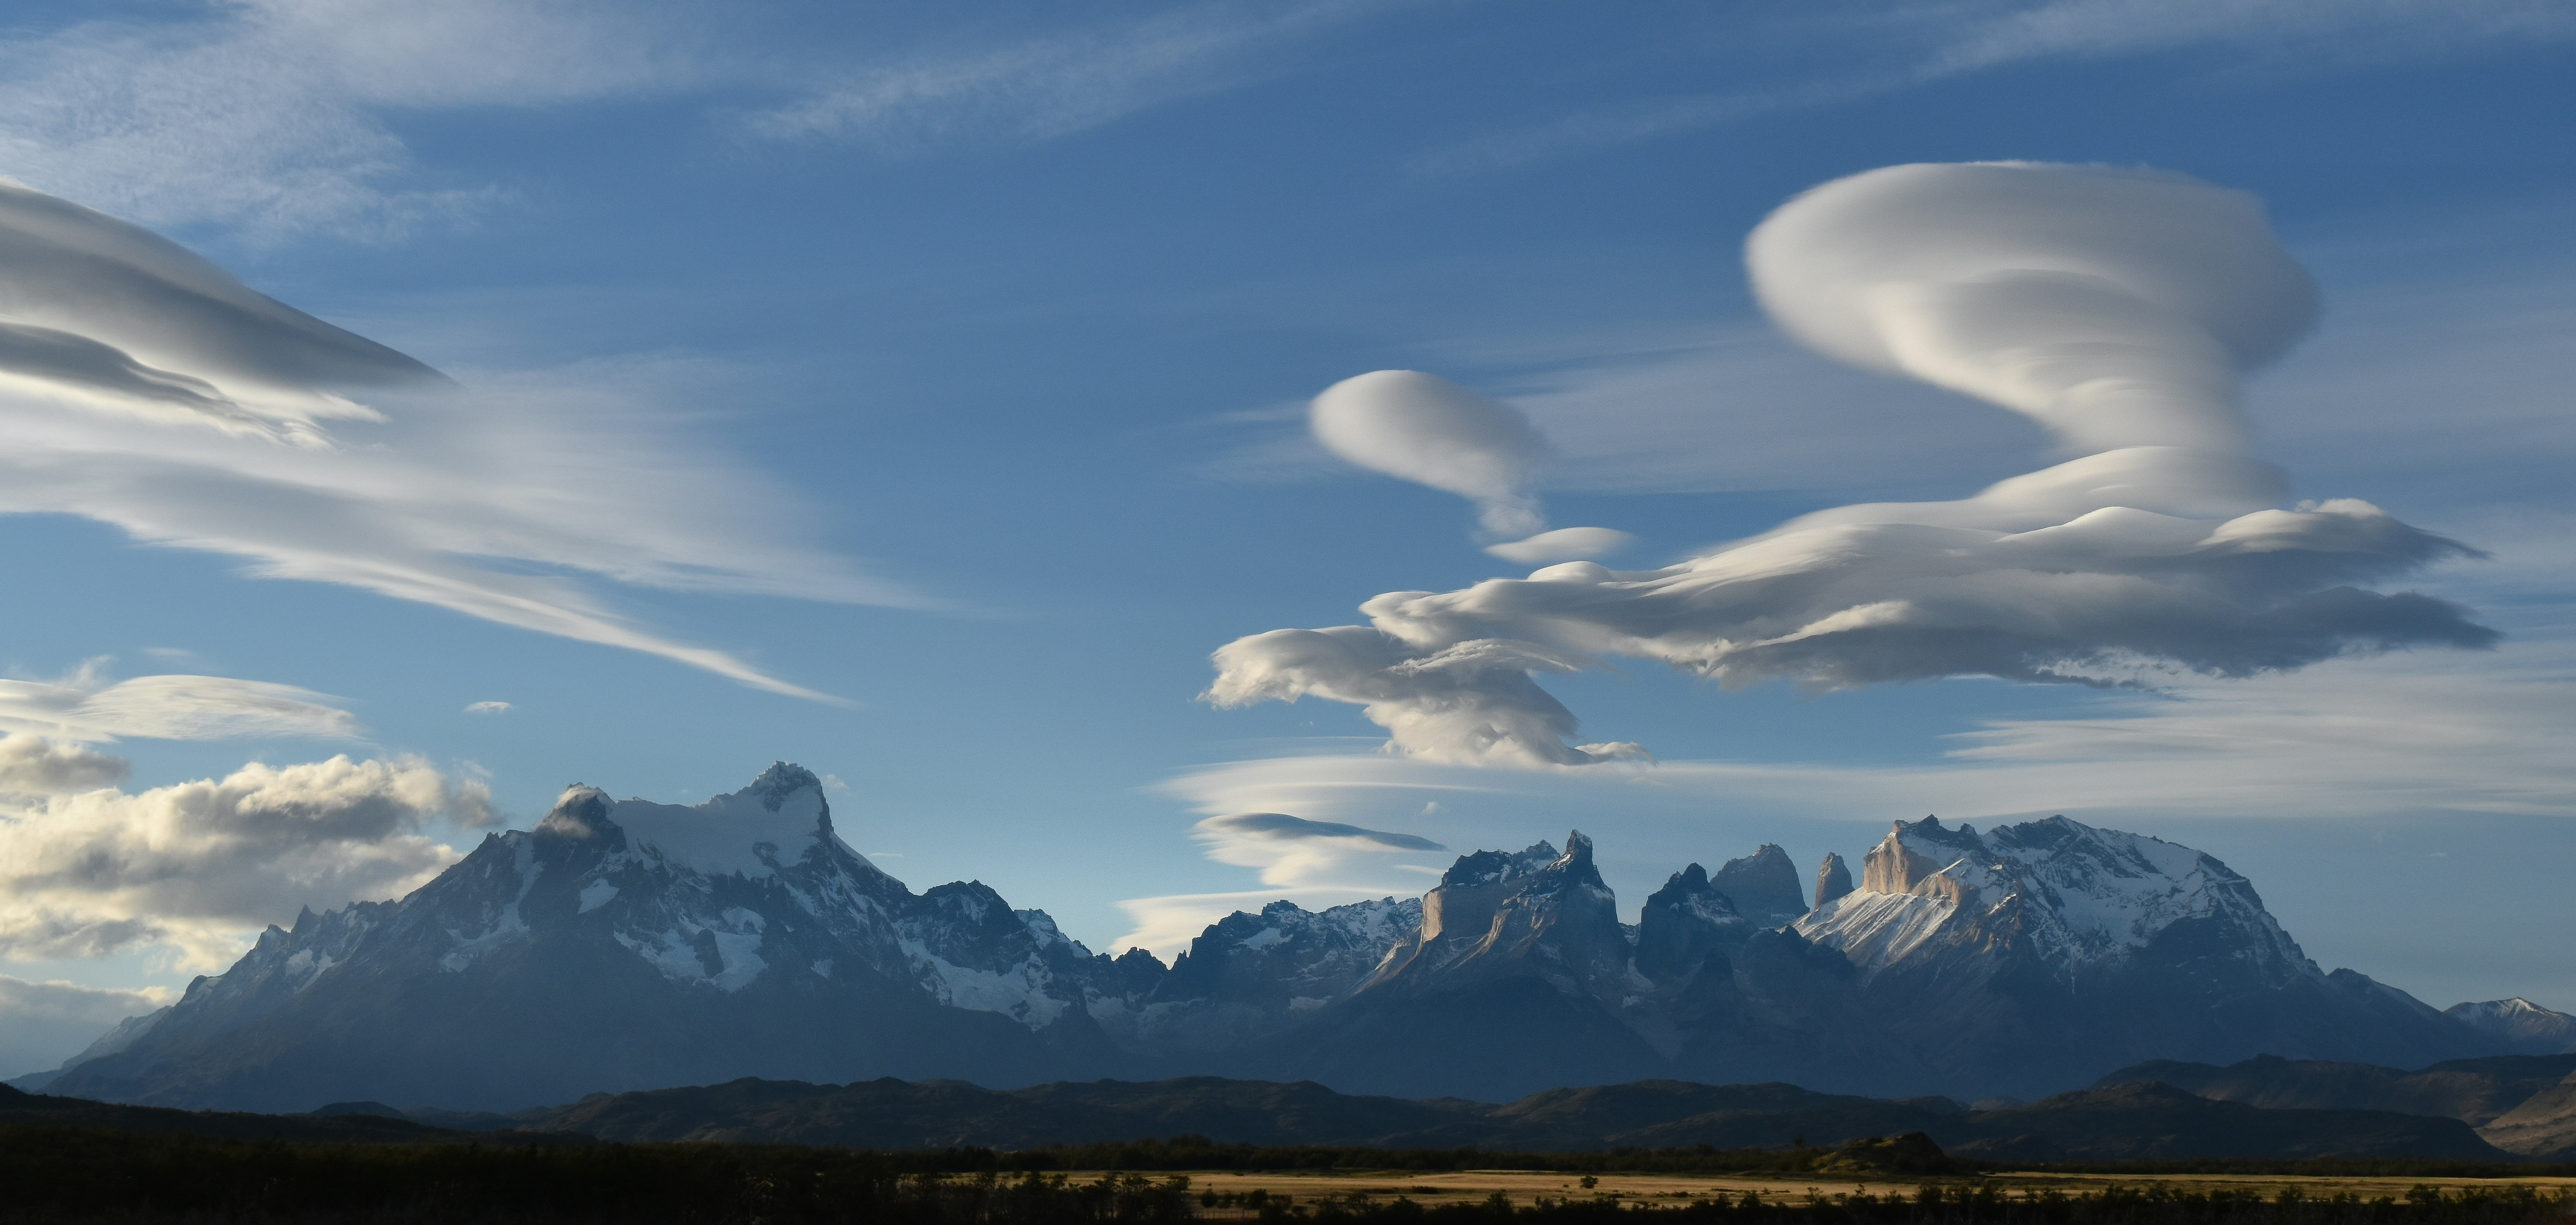
\includegraphics[width=\linewidth,height=\solofigbody,keepaspectratio]{figures/clouds.jpg}
		\vspace{0.5em}
		{\tiny \textit{Mountain waves. \href{https://unsplash.com/photos/white-clouds-over-mountains-during-daytime-I8CF-ST8WxE}{Source: Marc Thunis}}\par}
	\end{columns}
\end{frame}
\begin{frame}{Internal gravity wave prototype}
	\begin{itemize}
		\item \emph{air density} and \emph{atmospheric pressure} are stratified
		\item a displaced air parcel is pushed back by buoyancy \& gravity $\Rightarrow$ \textbf{internal gravity wave}
	\end{itemize}

	\vspace{0.5em}

	\begin{center}
		\resizebox{!}{135pt}{%
			\begin{tikzpicture}[node distance = 2cm]
				\node (A) [draw, align=center, text width=3.5cm] at (0,2) {\scriptsize an air parcel ascends to a region of lower density};
				\node (B) [draw, align=center, text width=3.5cm] at (3.5,0) {\scriptsize buoyancy decreases; gravity drives it downward};
				\node (C) [draw, align=center, text width=3.5cm] at (0,-2) {\scriptsize the parcel reaches a region of higher density};
				\node (D) [draw, align=center, text width=3.5cm] at (-3.5,0) {\scriptsize buoyancy increases; buoyancy force drives it upward};

				\draw[->,thick] (A) -- (B);
				\draw[->,thick] (B) -- (C);
				\draw[->,thick] (C) -- (D);
				\draw[->,thick] (D) -- (A);
			\end{tikzpicture}%
		}
	\end{center}
\begin{itemize}
	\item initial displacement caused by hitting the mountain profile
\end{itemize}
\end{frame}

\begin{frame}{Potential temperature $\theta$}
	\begin{columns}[c,onlytextwidth]
		\column{0.52\textwidth}
		\begin{itemize}
			\setlength{\itemsep}{1.2em}
			\item thermodynamic temperature a parcel would have if moved \textbf{adiabatically} from $(T, p)$ to $(\theta, p_0)$
			\item conserved under \emph{isentropic flows}
			\item \textbf{stratification stability condition}: $\partial_{z} \theta > 0$.
		\end{itemize}

		\vspace{1em}

		\begin{math-block}{Potential temperature expression}
			\begin{equations}[single,*,noskip]
				\theta = T \left(\frac{p_0}{p}\right)^{\frac{R}{c_p}}.
			\end{equations}
		\end{math-block}

		\column{0.43\textwidth}
		\centering
		% The parcel is drawn twice: solid where it actually is, dashed at the
		% reference pressure, because that lower state is hypothetical -- it is
		% the definition of theta, not a place the parcel has been.  No tikz
		% library needed: the blob is a smooth cycle through seven points.
		%
		% Labels sit above the isobars and the p_0 note below them rather than
		% out to the right: that keeps the drawing taller than it is wide (0.8),
		% so scaling it to the frame height rather than the column width is what
		% makes it big -- 136pt wide against the 171pt column, but the isobars
		% themselves are half again as long as they were in a width-scaled version.
		\resizebox{!}{170pt}{%
			\begin{tikzpicture}[x=1cm, y=1cm]
				% isobars
				\draw[thick, dashed, DragonGray] (-1.7,2.8) -- (1.7,2.8);
				\draw[thick, dashed, DragonGray] (-1.7,0)   -- (1.7,0);
				\node[above right, SumiInk] at (0.55,2.85) {$(T, p)$};
				\node[above right, SumiInk] at (0.55,0.05) {$(\theta, p_0)$};

				% the parcel where it is
				\begin{scope}[shift={(-0.7,2.8)}]
					\draw[DragonTeal, thick, fill=DragonTeal!20]
						plot[smooth cycle] coordinates
						{(0,0.45) (0.45,0.28) (0.6,-0.1) (0.2,-0.45)
						 (-0.35,-0.35) (-0.6,0.05) (-0.35,0.38)};
				\end{scope}

				% the same parcel brought down to p_0
				\begin{scope}[shift={(-0.7,0)}]
					\draw[DragonTeal, thick, dashed, fill=DragonTeal!8]
						plot[smooth cycle] coordinates
						{(0,0.45) (0.45,0.28) (0.6,-0.1) (0.2,-0.45)
						 (-0.35,-0.35) (-0.6,0.05) (-0.35,0.38)};
				\end{scope}

				\draw[->, thick, DragonRed] (-0.7,2.2) -- (-0.7,0.6)
					node[midway, right=3pt, font=\small, DragonGray] {adiabatic};

				\node[below, DragonGray, font=\small] at (0,-0.85)
					{$p_0 = \SI{1013.25}{\hecto\pascal}$};
			\end{tikzpicture}%
		}
	\end{columns}
\end{frame}
\section{Mathematical description}
\label{sec:MATH}
\begin{frame}{Governing equations}
	\begin{math-block}{Compressible isentropic Euler equations}
		\begin{equations}[columns,*]
			\rho \dv{\vb{v}}{t} &= -\grad p + \rho \vb{g},                && \eqnote{momentum balance} \\
			\dv{\rho}{t} + \rho\left(\divergence{\vb{v}}\right) &= 0,     && \eqnote{mass conservation} \\
			\dv{\theta}{t} &= 0,                                      && \eqnote{isentropic evolution, $\theta = T \left(\frac{p_0}{p}\right)^{\frac{R}{c_p}}$} \\
			p\left(\rho, T\right) &= \rho R T.                     && \eqnote{thermal equation of state of an ideal gas}
		\end{equations}
	\end{math-block}
\end{frame}

\begin{frame}{Initial conditions}
	\begin{math-block}{Isothermal hydrostatic balance, $T_0 = \SI{250}{\kelvin}$}
		\begin{equations}[columns,*]
			\vb{v}\left(0, \vb{x}\right) &= \vb{0},\\
			\rho\left(0, \vb{x}\right) &= \bar{\rho}(z) \coloneq \rho_0 \exp\left(-z \frac{g}{R T_0}\right), \\
			\theta\left(0, \vb{x}\right) &= \bar{\theta}(z) \coloneq T_0 \exp\left(z\frac{R}{c_p}\frac{g}{R T_0}\right), \\
			p\left(0, \vb{x}\right) &= \bar{p}(z) \coloneq \rho_0 R T_0 \exp\left(-z \frac{g}{R T_0}\right) && \eqnote{ $\Leftarrow$ equation of state}.
		\end{equations}
	\end{math-block}
\end{frame}

\begin{frame}{Domain \& boundary conditions}
	\begin{columns}[T,onlytextwidth]
		\begin{column}{0.5\textwidth}
			$ \Omega \subset \mathbb{R}^2, \partial \Omega = \Gamma_{\, \text{west} \,} \cup \Gamma_{\, \text{east} \,} \cup \Gamma_{\, \text{bot} \,} \cup \Gamma_{\, \text{top} \,}$
			\begin{math-block}{Imposed boundary conditions}
				\begin{equations}[columns,*]
					\vb{v} &= v_0 \vb{e}_x \, \text{on} \, \Gamma_{\, \text{west} \,}, && \eqnote{subsonic inflow: $v_0 < c$} \\
					\theta &= \bar{\theta}\left(z\right), \, \text{on} \, \Gamma_{\, \text{west} \,}, && \eqnote{hydrostatic profile} \\
					\vb{v} \vdot \vb{n} &= 0 \, \text{on} \, \Gamma_{\, \text{bot} \,}, && \eqnote{no-penetration}\\
					p &= \bar{p}\left(z\right) \, \text{on} \, \Gamma_{\, \text{east} \,},  && \eqnote{subsonic outflow}\\
				\end{equations}
			\end{math-block}
			\vspace{0.5em}

			together with the \emph{radiation boundary condition} on the \emph{artificial} boundary $\Gamma_{\, \text{top} \,}$.
			\vspace{1em}
		\end{column}

		\begin{column}{0.45\textwidth}
			\centering

			\resizebox{\textwidth}{!}{%
				\begin{tikzpicture}[scale=1, every node/.style={transform shape}]
					% Boundaries
					\draw[thick, blue] (-3,0.5) -- (-3,3.5); 
					\node[left, black, font=\small] at (-3, 1) {$\Gamma_{\text{west}}$};
					\draw[->, thick] (-4.3, 2) -- (-3.4, 2)
					node[midway, above, inner sep=2pt] {$\vb{v} = v_0\vb{e}_x$}
					node[midway, below, inner sep=2pt] {$\theta = \bar{\theta}(z)$};

					\draw[thick, red] (3,0.5) -- (3,3.5);
					\node[right, black, font=\small] at (3, 1) {$\Gamma_{\text{east}}$};
					\node[right, black, font=\small] at (3, 2) {$p = \bar{p}(z)$};

					\draw[thick, gray, dashed] (-3,3.5) -- (3,3.5)
					node[midway, above, black, font=\small, align=center]
					{radiation boundary condition \\ $\Gamma_{\text{top}}$};

					\draw[thick, brown, domain=-3:3, samples=100] plot (\x, {0.5 + 1.5/( \x*\x + 1 )});
					\node[below, black, font=\small, align=center] at (0,0.5)
					{$\Gamma_{\text{bot}}$ \\ $\vb{v} \vdot \vb{n} = 0$};

					\node at (0,2.5) {\Large $\Omega$};

				\end{tikzpicture}%
			}

			\vspace{0.5em}

			\resizebox{0.824\textwidth}{!}{% same scale as the sketch above (see note there)
				\begin{tikzpicture}
					\begin{axis}[
						xlabel={$x$ (km)},
						ylabel={$h(x)$ (m)},
						xlabel style={anchor=north east},  
						ylabel style={anchor=south east},  
						xmin=-200, xmax=200,
						ymin=0, ymax=110, 
						xtick={-200,-100,0,100,200},  
						ytick={0,25,50,75,100},  
						axis lines=middle,
						width=8cm, 
						height=5cm,
						]
						\addplot[thick, black, domain=-200:200, samples=200] {10000/(x^2 + 100)};
					\end{axis}
				\end{tikzpicture}%
			}
		\end{column}
	\end{columns}
\end{frame}

\section{Numerical solution}
\label{sec:NUMERICS}
\begin{frame}{Smoothed Particle Hydrodynamics}
	\begin{itemize}
		\item fluid is partitioned into \emph{abstract material points} $\{\vb{x}_a\}$, so called \textbf{particles}
	\item equations are discretised using an \textbf{interpolation kernel} $w_h\left(\vb{x}\right), h \propto \mathrm{diam} \, \mathrm{supp} w_h$
	\end{itemize}

	\begin{equations}[columns,*]
		\uncover<2->{\Phi\qty(t,\vb{x}) = \Phi\qty(t,\vb{x}) \star \delta\qty(\vb{x})} &\uncover<2->{=\int_{\Omega}\Phi\qty(t,\vb{x}') \delta\qty(\vb{x}-\vb{x}')\dd{\vb{x}'} \Rightarrow} && \uncover<2->{\eqnote{convolution identity}} \\
		\uncover<3->{[\Phi]^C_{w_h}\qty(t,\vb{x}) \coloneq \Phi\qty(t,\vb{x}) \star w_h\qty(\vb{x})} &\uncover<3->{= \int_{\Omega}\Phi\qty(t,\vb{x}')w_h\qty(\vb{x}-\vb{x}')\dd{\vb{x}'},} && \uncover<3->{\eqnote{continuous interpolation}} \\
		\uncover<4->{[\Phi]_{w_h}^C(t,\vb{x}_a)} &\uncover<4->{\approx \sum_{\vb{x}_b \in \mathrm{supp}w_h} \Phi\left(t, \vb{x}_b\right) w_h\left(\vb{x}_a - \vb{x}_b\right) V_b \coloneq \Phi_a\left(t\right),} && \uncover<4->{\eqnote{discrete interpolation}}\\
		\uncover<5->{\Phi(t,\vb{x}_a)} &\uncover<5->{\approx [\Phi]_{w_h}^C\qty(t,\vb{x}_a) \approx \Phi_a(t).} && \uncover<5->{\eqnote{particle approximation}}
	\end{equations}

	\begin{itemize}
		\item<6-> the resulting system of \emph{ODEs} is solved numerically using a \textbf{symplectic integrator}
	\end{itemize}
\end{frame}

\begin{frame}{Why SPH?}
	\begin{itemize}
		\item \textbf{conservative} properties, accessible \textbf{trajectories}
	\end{itemize}

	\solofigure{figures/divergence.png}{Reference results: vertical component of the velocity field \href{https://doi.org/10.1175/MWR-D-10-05042.1}{Monthly Weather Review 139, 9; 10.1175/MWR-D-10-05042.1}}{fig:WHY}
\end{frame}

\begin{frame}{$p-\theta$ formulation}
	\begin{columns}[T,onlytextwidth]
		\column{0.4\textwidth}
		\centering
		\begin{math-block}{Classical SPH}
			\begin{equations}[columns,*]
				\dv{\rho_a}{t} &= \sum_b m_b w'_{ab} \vb{v}_{ab}\vdot \vb{e}_{ab}, \\
				\dv{\vb{v}_a}{t} &= -\sum_b m_b \qty(\frac{p_a}{\rho_a^2}+\frac{p_b}{\rho_b^2})w'_{ab}\vb{e}_{ab} + \vb{g}, \\
				\theta &= T_a \left(p_0/p_a\right)^{\frac{R}{c_p}} \approx \, \text{const} \,,
			\end{equations}
		\end{math-block}
		\begin{itemize}
			\item poor conservation properties with \link[h]{adaptive $h$},
			\item $\theta$ has to be computed at extra cost.
		\end{itemize}

		\column{0.55\textwidth}
		\centering
		\begin{math-block}{Novel $p-\theta$ formulation}
			\begin{equations}[columns,*]
				p_a &= \left(\sum_{b} \frac{m_b}{\tilde{\theta_0}} \theta_b w_{ab}\left(\link[h]{h_a}\right)\right)^{\gamma},\\
				\dv{\vb{v}_a}{t} &= - \sum_{b} m_b \frac{\theta_a \theta_b}{\tilde{\theta}_0^{2}}\left(\frac{\link[f]{f_{a}}p_a}{p_a^{2/\gamma}} w'_{ab}\left(\link[h]{h_a}\right) + \frac{\link[f]{f_{b}}p_b}{p_b^{2/\gamma}} w'_{ab}\left(\link[h]{h_b}\right)\right)\vb{e}_{ab} + \vb{g},\\
				\theta_a &= \, \text{const} \,
			\end{equations}
		\end{math-block}
		\begin{itemize}
			\item naturally guarantees conservation with \link[h]{adaptive $h$} via the $\link[f]{\grad h}$ \link[f]{terms} $\link[f]{f_{a}}$,
			\item uses the primary variable $\theta$ directly.
		\end{itemize}
	\end{columns}
\end{frame}

\begin{frame}{Well-balanced SPH formulations}
	\begin{itemize}
		\item hydrostatic $\bar{\rho}, \bar{p}$ solve
	\end{itemize}

	\begin{equations}[single,*,noskip]
		\cancel{\bar{\rho} \dv{\vb{v}}{t}} + \grad \bar{p} - \bar{\rho} \vb{g} = \vb{0},
	\end{equations}

	\begin{itemize}
		\item<2-> general numerical approximations $\bar{\rho_h}, \bar{p_h}, \grad_h$
	\end{itemize}

	\begin{equations}[single,*,noskip]
		\uncover<2->{\grad_h \bar{p_h} - \bar{\rho_h} \vb{g} \neq \vb{0} \Rightarrow \, \text{\textbf{spurious force}} \,}
	\end{equations}

	\uncover<2->{%
		\begin{alert-block}
			Hydrostatic balance does not generally hold on the discrete level!
		\end{alert-block}
	}

	\begin{itemize}
		\item<3-> \textbf{well-balanced scheme}: stationary states preserved \textbf{after discretisation}
	\end{itemize}

	\uncover<3->{%
	\begin{math-block}{Well-balancing: substituting for gravity}
		\begin{equations}[single,*,noskip]
			\vb{g} = \frac{1}{\bar{\rho}} \grad \bar{p} \Rightarrow \dv{\vb{v}}{t} = - \frac{1}{\rho} \grad p + \frac{1}{\bar{\rho}} \grad \bar{p}
		\end{equations}
	\end{math-block}
	}

	\begin{itemize}
	\item<3-> identical discretisation of gradients $\Rightarrow$ identical truncation errors $\Rightarrow$ they \textbf{subtract}
	\end{itemize}
\end{frame}

\section{Results}
\label{sec:RESULTS}

\begin{frame}{The failure of classical SPH: velocity field}
	\solofigure{figures/results/field_SPH.png}{Nonzero velocity field computed by classical SPH - a failure of hydrostatic balance.}{fig:SPH_FIELD}
\end{frame}

\begin{frame}{The failure of classical SPH: velocity norms}
	\solofigure{figures/results/norms_SPH.png}{Nonzero norms of the velocity field - a failure of hydrostatic balance}{fig:SPH_NORMS}
\end{frame}

\begin{frame}{The success of well-balanced $p-\theta$: velocity field}
	\solofigure{figures/results/field_WB.png}{Caption.}{fig:WB_FIELD}
\end{frame}

\begin{frame}{The success of well-balanced $p-\theta$: velocity norms}
	\solofigure{figures/results/norms_PTH.png}{Caption.}{fig:WB_NORMS}
\end{frame}

\begin{frame}{Partial success: emergence of a wave}
	\panelgrid[3]{%
		\panel{figures/results/wave_1.png}{$t = \SI{360}{\second}$}
		\panel{figures/results/wave_2.png}{$t = \SI{420}{\second}$}
		\panel{figures/results/wave_3.png}{$t = \SI{480}{\second}$}
		\panel{figures/results/wave_4.png}{$t = \SI{540}{\second}$}
		\panel{figures/results/wave_5.png}{$t = \SI{600}{\second}$}
		\panel{figures/results/wave_6.png}{$t = \SI{660}{\second}$}
	}
\end{frame}

\begin{frame}{Tensile instability: clustering}
	\solofigure{figures/results/instab_02.png}{$t = \SI{690}{\second}$}{fig:INSTAB1}
\end{frame}

\begin{frame}{Tensile instability: explosion}
	\solofigure{figures/results/instab_05.png}{$t = \SI{710}{\second}$}{fig:INSTAB2}
\end{frame}

\begin{frame}{Tensile instability: breakdown}
	\solofigure{figures/results/instab_07.png}{$t = \SI{720}{\second}$}{fig:INSTAB3}
\end{frame}

\begin{frame}{Summary}
	\begin{columns}[c,onlytextwidth]
		\column{0.42\textwidth}
		\begin{itemize}
			\setlength{\itemsep}{1.2em}
			\item flows around a topography induce internal gravity waves
			\item IGWs play a significant role in mesoscale atmospheric dynamics
			\item large scale hydrostatic balance is problematic for classical SPH
			\item well-balanced schemes with adaptive smoothing lengths must be used for non-stationary flows
		\end{itemize}
		\column{0.55\textwidth}
		\centering
		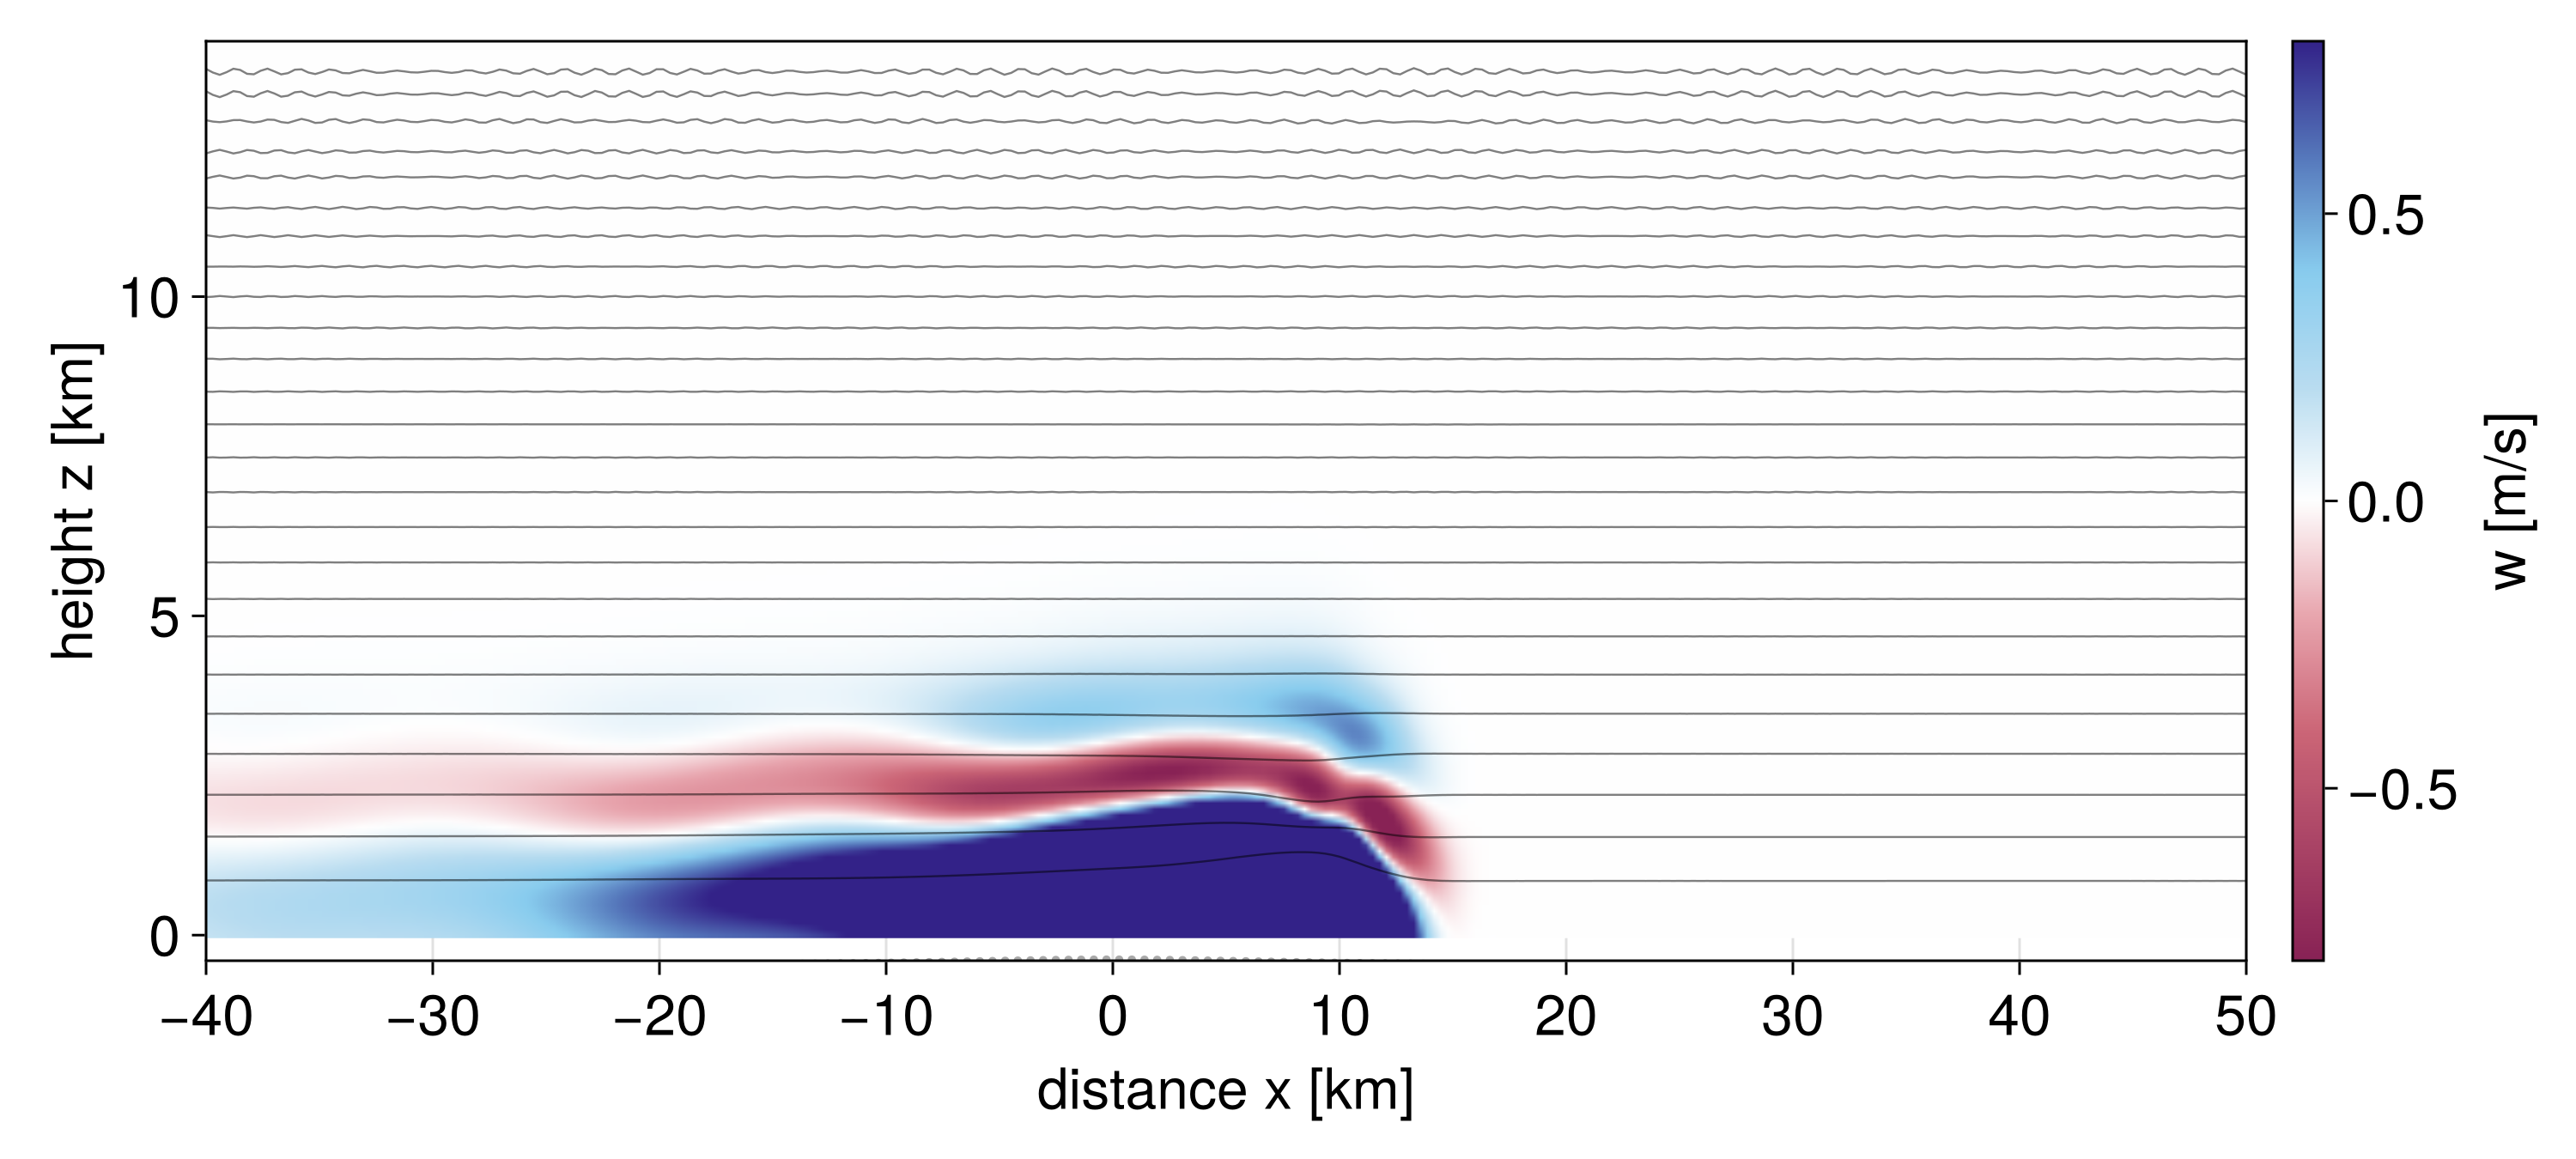
\includegraphics[width=\linewidth,height=\solofigbody,keepaspectratio]{figures/results/wave_5.png}
	\end{columns}
\end{frame}

\begin{frame}{Future plans}
	\begin{columns}[c,onlytextwidth]
		\column{0.42\textwidth}
		\begin{itemize}
			\setlength{\itemsep}{1.2em}
			\item resolve tensile instability by $\delta-$SPH regularization
			\item implement other boundary conditions, include real topography
			\item compare the results with the analytic solution
			\item compare the results with other models \& methods.
		\end{itemize}
		\column{0.55\textwidth}
		\centering
		% the credit line below the plot is what the 16pt buys back
		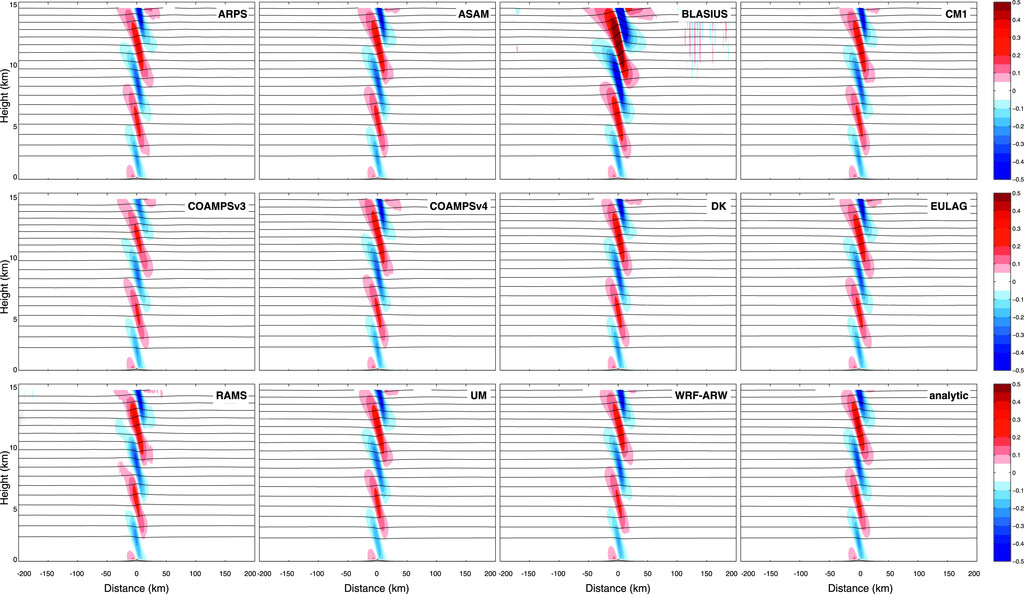
\includegraphics[width=\linewidth,height=\dimexpr\solofigbody-16pt\relax,keepaspectratio]{figures/reference.jpg}
		\vspace{0.5em}
		{\tiny \textit{Reference results. \href{https://doi.org/10.1175/MWR-D-10-05042.1}{Monthly Weather Review 139, 9; 10.1175/MWR-D-10-05042.1}}\par}
	\end{columns}
\end{frame}
\appendix
\selectlanguage{czech}

\section{Reakce na otázky z posudků}
\label{sec:RESPONSES}

\begin{qaframe}{Oponent, otázka 1}
	\begin{question}
		Vztah (2.4), uvažovala/testovala se i jiná volba okrajových podmínky na vstupu a výstupu, viz komentář v práci na str. 27?
	\end{question}

	% \begin{answer}
	% \end{answer}
\end{qaframe}

\begin{qaframe}{Oponent, otázka 2}
	\begin{question}
		Numerické experimenty v Kapitole 6 potvrzují schopnost metody zachovávat stacionární stavy. Částečně však postrádám další numerické verifikace, např. vyšetřování přesnosti či stability metody. Byly prováděny též experimenty v této oblasti?
	\end{question}

	% \begin{answer}
	% \end{answer}
\end{qaframe}

\begin{qaframe}{Oponent, otázka 3}
	\begin{question}
		Na základě zkušeností s řešením práce, jaký je potenciál částicových metod ve srovnání se \uv{sítovými metodami} (FEM, FVM, DG) pro řešení komplikovanějších 3D úloh?
	\end{question}

	% \begin{answer}
	% \end{answer}
\end{qaframe}

\begin{qaframe}{Vedoucí, otázka 1}
	\begin{question}
		Dá se pozorovaná vertikální vlna nazvat gravitační vlnou v meteorologickém kontextu?
	\end{question}

	% \begin{answer}
	% \end{answer}
\end{qaframe}

\begin{qaframe}{Vedoucí, otázka 2}
	\begin{question}
		Dal by se proměnlivý kernel začlenit do hamiltonovské formulace?
	\end{question}

	% \begin{answer}
	% \end{answer}
\end{qaframe}

\begin{qaframe}{Vedoucí, otázka 3}
	\begin{question}
		Jak obtížné by bylo vyvinout well-balanced implementaci SPH s $\delta-$SPH regularizací?
	\end{question}

	% \begin{answer}
	% \end{answer}
\end{qaframe}

\end{document}
